\documentclass[12pt]{article}

\usepackage{graphicx}
\usepackage{paralist}
\usepackage{amsfonts}
\usepackage{hyperref}
\usepackage{listings}
\usepackage{subfig}

\oddsidemargin 0mm
\evensidemargin 0mm
\textwidth 160mm
\textheight 200mm
\renewcommand\baselinestretch{1.0}

\pagestyle {plain}
\pagenumbering{arabic}
\newcounter{stepnum}

\title{Course Project}
% \author{Hyosik Moon}

\begin {document}

\maketitle

\section{Required}

\begin{itemize}
\item \textbf{Main objective of the analysis} \\
I will analyze the World Happiness Report. 
It quantified the level of happiness from 0 (Worst) to 10 (Happiest). To be specific, 1) we will get the best linear regression model to predict the level of happiness with features, and 2) we will take a closer look at what features have a significant impact on the level of happiness.

\item \textbf{Brief description of the data set} \\
The happiness scores and rankings use data from the Gallup World Poll. There are 149 rows (objects, countries), and 20 columns (features). The target is Ladder score which is the numeric indicator of the level of happiness. And there are two categorical features that are 'Country name', and 'Regional indicator'. (Figure \ref{descr}, \ref{categ})



\begin{figure}[hbt!]
    \centering
    \subfloat[Numerical variables]{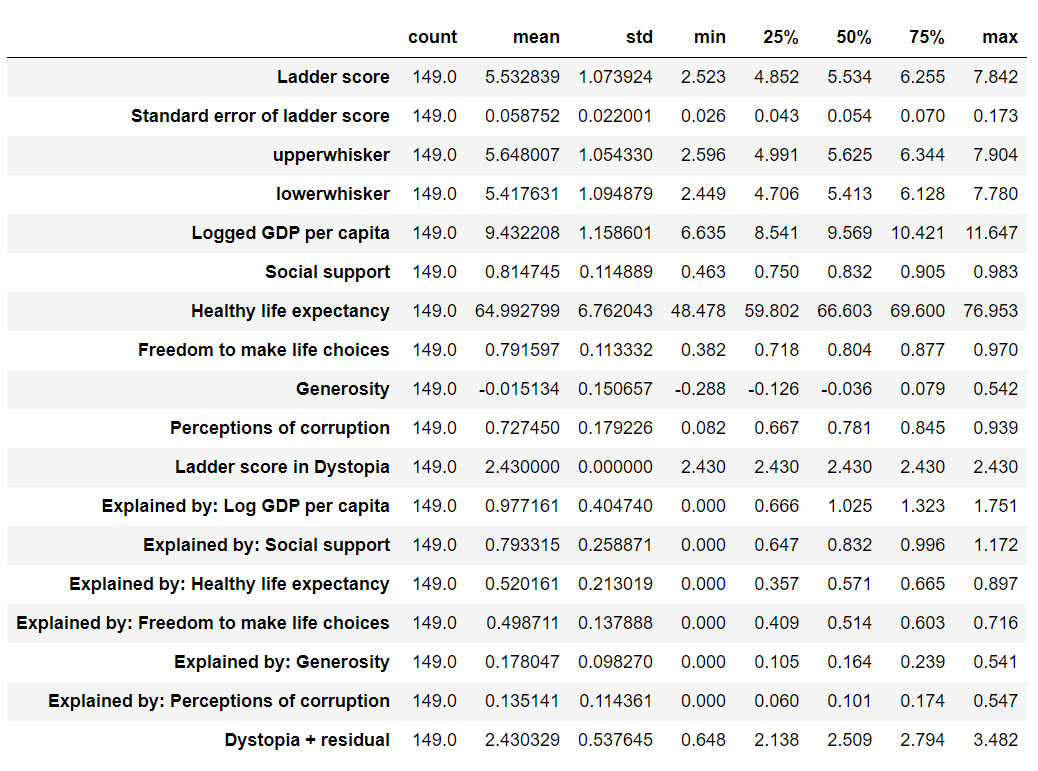
\includegraphics[width=0.63\textwidth]{figures/data_description.png}\label{descr}}
    \hfill
    \subfloat[Categorical variables]{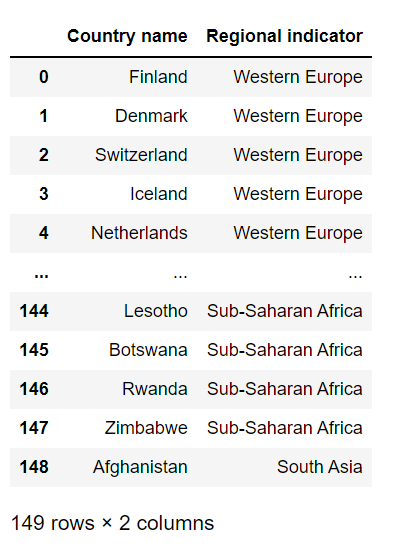
\includegraphics[width=0.37\textwidth]{figures/categorical_var.png}\label{categ}}
    \caption{Brief description of the data set}
\end{figure}

\item \textbf{Brief summary of data exploration}
    \begin{enumerate}
    \item Data cleaning, Delete unused features to predict the Ladder score.
    \item Plot the relationship between Ladder score and other variables and find the higher-correlation features (Figure \ref{pairplot}). According to pairplot, the Generosity seems not to have a strong correlation.
    
    \begin{figure}[hbt!]
        \centering
        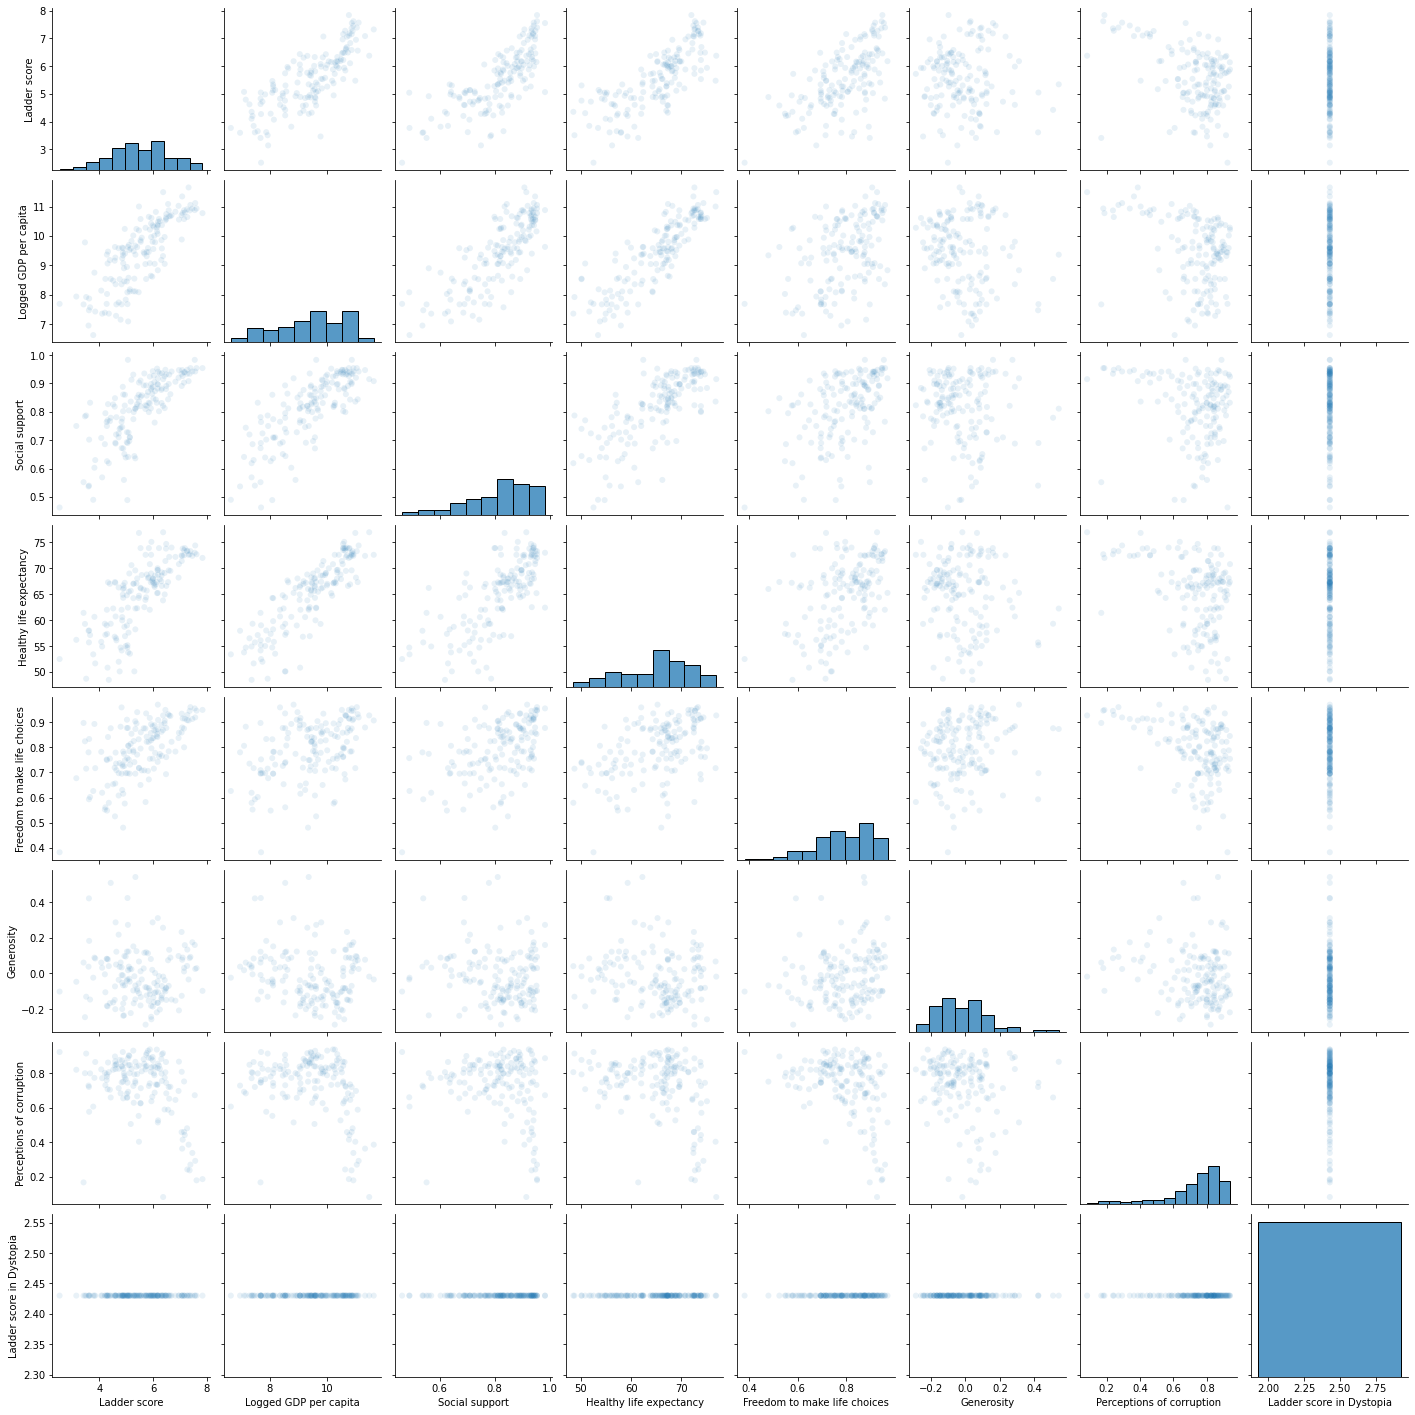
\includegraphics[width=0.9\textwidth]{figures/pairplot.png}
        \caption{Pair plots among features}\label{pairplot}
    \end{figure}
    
    \item Change the categorical variable to numeric variables. (Figure \ref{ohc})
    
    \begin{figure}[hbt!]
        \centering
        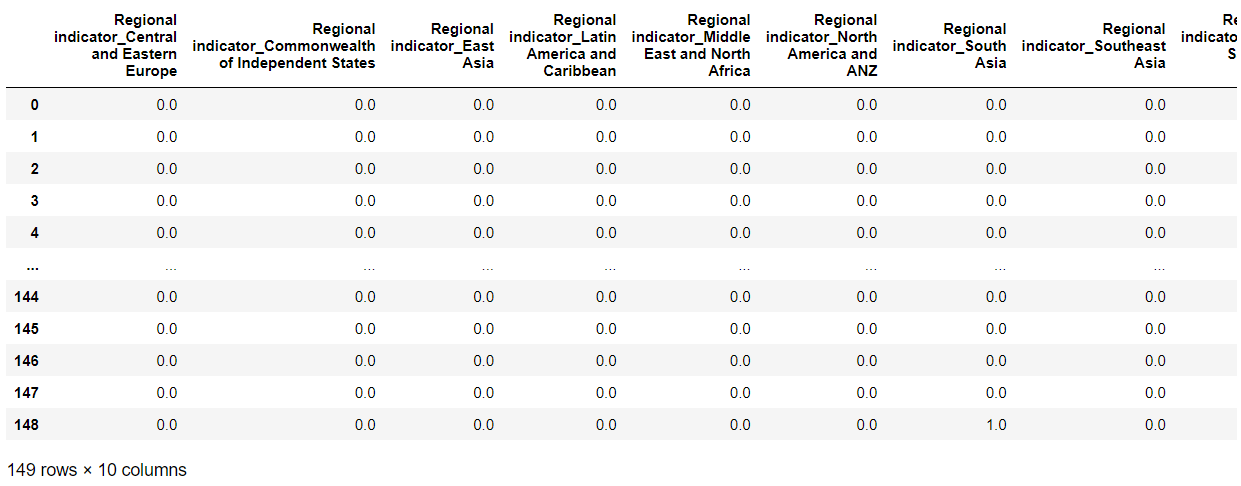
\includegraphics[width=0.8\textwidth]{figures/ohc.png}
        \caption{OneHotEncoder}\label{ohc}
    \end{figure}

    \item Standardize the features. (Figure \ref{std})

    \begin{figure}[hbt!]
        \centering
        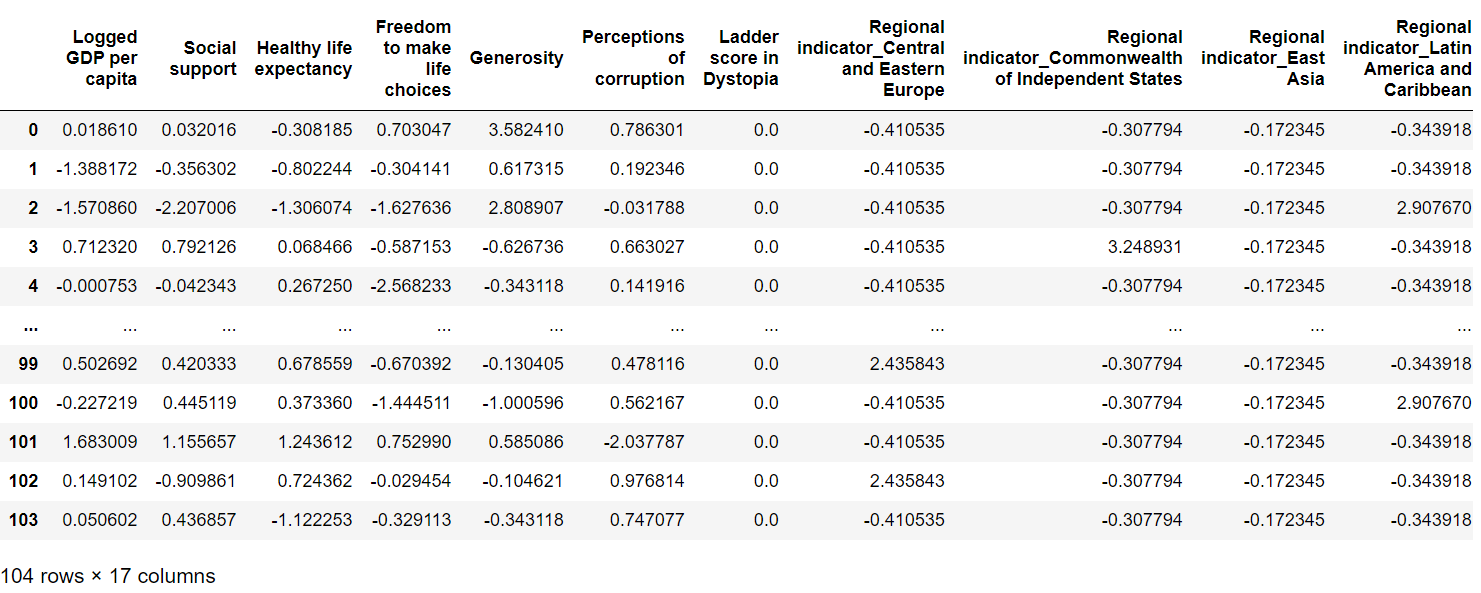
\includegraphics[width=0.8\textwidth]{figures/std.png}
        \caption{Standardized values}\label{std}
    \end{figure}

    \item Check the normality of the target value and normalize if it's skewed. \\
    \textit{Ladder score}'s p-value is 0.526. So, we don't need to normalize the target value. (Figure \ref{nom})

    \begin{figure}[hbt!]
        \centering
        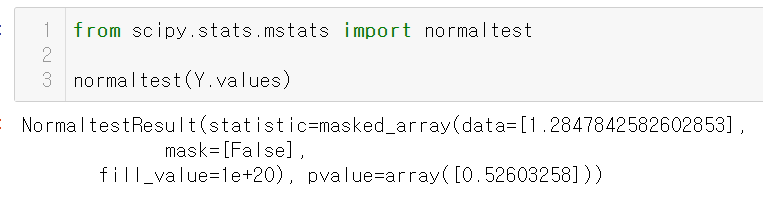
\includegraphics[width=0.8\textwidth]{figures/normalize.png}
        \caption{Check the normality of the target}\label{nom}
    \end{figure}
    
    \end{enumerate}

\item \textbf{Summary of training at least three linear regression models}
We tested 4 kinds of models such as \textit{Linear Regression, Lasso, Ridge, ElasticNet} and in order to prevent overfitting we used cross validation. To evalueate the best model, we compare the results with rmse(root mean squared error). This is the result of rmse of the four models. (Figure \ref{rmse})

\begin{figure}[hbt!]
    \centering
    \includegraphics[width=0.4\textwidth]{figures/rmse.png}
    \caption{Check the rmse of the models}\label{rmse}
\end{figure}

\item \textbf{Explanation of your final regressions model}
Overall, all models showed the low rmse values. But the best one was Ridge $(ridgeCV.alpha\_ :  21.056578947368422  ridgeCV\_rmse:  0.501828479703691)$. And the r2\_score of the model was $0.7610082843481112$.

\item \textbf{Summary Key Findings and Insights}
When we analyze the coefficients, it shows the interesting result. The regions are the main fators that people feel happy. I think it's resonable because happiness is decided based on the relationship. So, some regions might have a culture that put big emphasis on the relationship (Figure \ref{factors})

\begin{figure}[hbt!]
    \centering
    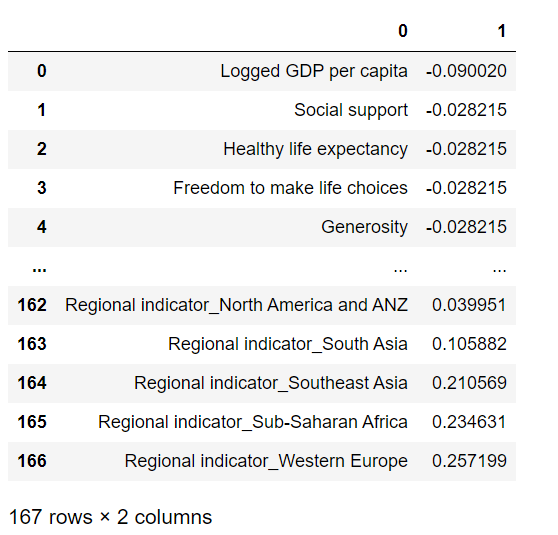
\includegraphics[width=0.8\textwidth]{figures/factors.png}
    \caption{Coefficients. Regions are the main factors}\label{factors}
\end{figure}

\item \textbf{Suggestions for next steps}
We may find more meaningful results if we exclude the regions to predict the target. Because regions can be the result of different features such as GDP, Healthy, Social support, etc. Then, we will know the factor that has the most impact on the happiness rather than the regions.

\end{itemize}

\end {document}